
\documentclass[11pt]{article}
\usepackage[utf8]{inputenc}
\usepackage[french]{babel}
\usepackage{graphicx}
\usepackage[T1]{fontenc}
%\usepackage{amss}
\usepackage{amsmath}
\usepackage{amsfonts}
\usepackage{amssymb}

\newcommand\comment{}
\def\N{\mathbb N}
\def\R{\mathbb R}
\def\Q{\mathbb Q}
\def\Z{\mathbb Z}
\def\ie{{\it ie} }
\begin{document}
\title{EXAMEN I31, 2015}
\date{}\maketitle

{\bf La clarté et la concision de vos réponses est essentielle.}

{\bf Lisez l'énoncé avant de répondre. }

{
\section{Euclide et Bézout}
Pour $a=a_0=108, b=b_0=46$. 

Première question. Calculez le PGCD $g$  de $a$ et $b$, ainsi que $u\in\Z$ et $v\in \Z$, de norme minimale,
tels que $au+bv=g$.
Avant de remplir le tableau~:
$$\begin{array}{|c|c|c|c|c|c|c|c|}
\hline
i & a_i & b_i & a_i\div b_i & a_i\mbox{ mod }b_i & g_i &u_i & v_i \\
\hline
0 & 108 & 46 & ? & ? & ? & ? & ? \\
1 & ? & ? & ? & ? & ? & ? & ?  \\
2 & ? & ? & ? & ? & ? & ? & ?  \\
 &  &  &  &  &  &  &   \\
n & ?  & ? & ? & ? & ? & ? & ?  \\
\hline
\end{array}
$$
vous  définirez $u_i$ et $v_i$ en fonction de $u_{i+1}$ et $v_{i+1}$.

Deuxième question. Dans la dernière ligne, $n$,  du tableau (quand 
$b_n =0$), vous utiliserez $u_n=1$ et $v_n=k$, où $k\in\Z$ est une variable. 
Vous exprimerez tous les $u_i, v_i$ comme des fonctions de $k$.
Ceci vous donnera à la  ligne 0~: $u_0(k)$ et $v_0(k)$
tels que~: $108\times  u_0(k) + 46 \times v_0(k) = g$. 
}

\section{Dates au plus tôt et au plus tard}

Ce graphe est acyclique. Chaque sommet représente un état d'avancement de travaux~; chaque arc $s\rightarrow t$ représente une tâche, qu'il faut effectuer pour passer de l'état $s$ à l'état $t$. Les arcs sont étiquetés avec la durée 
de la tâche. 
Indiquez les dates au plus tôt et au plus tard 
de  chaque sommet (date au plus tôt --- au plus tard)
et soulignez le chemin critique.  
Par convention, la date au plus tôt du sommet source est 0.

\begin{center}
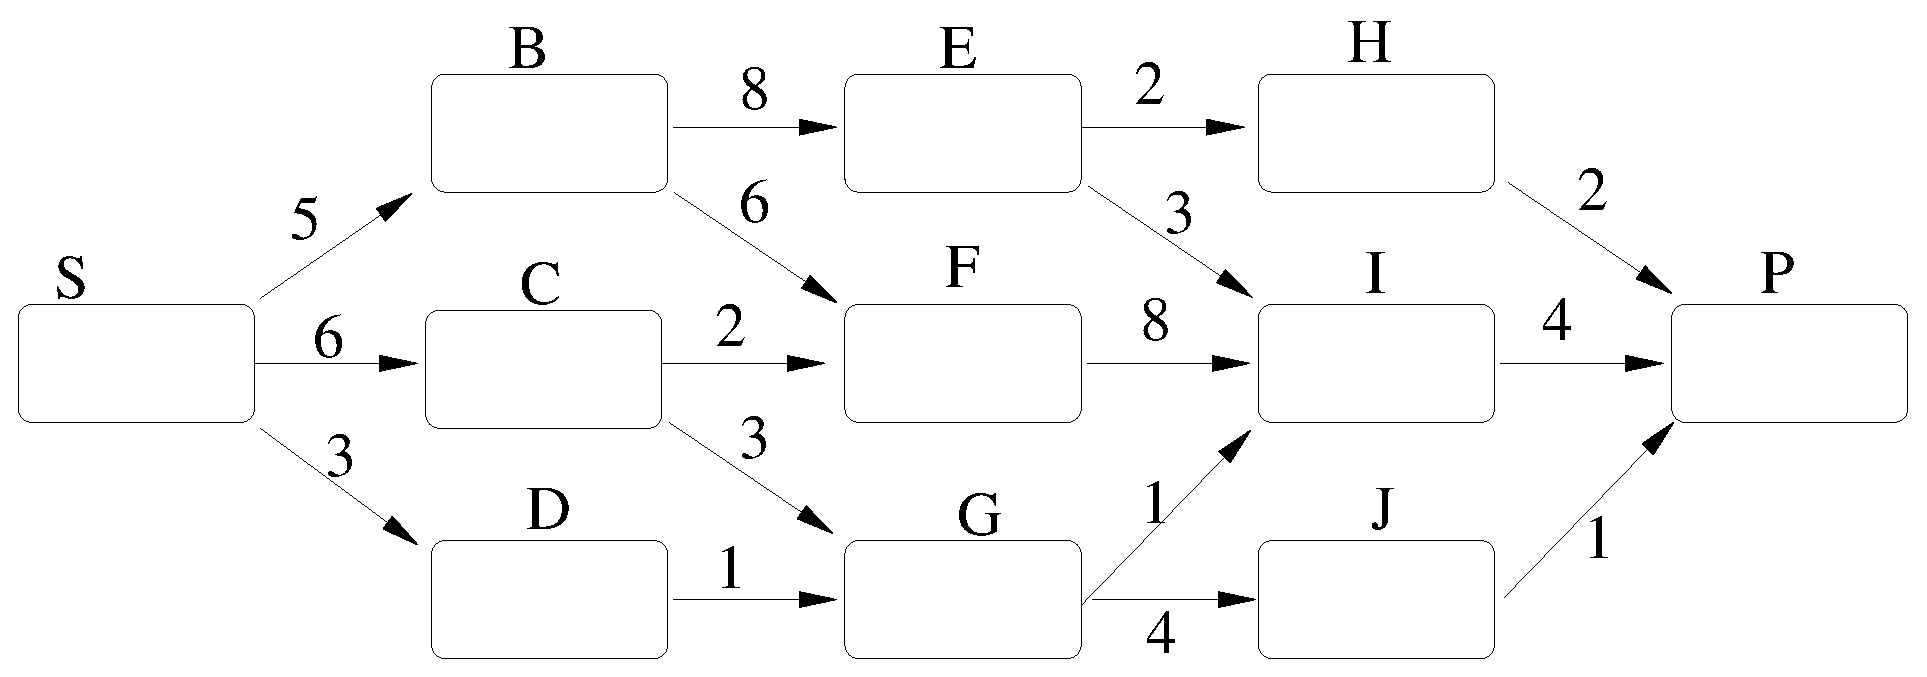
\includegraphics[width=0.9\linewidth]{critic.eps}
\end{center}



 

\section{Quizz}


1. Citez deux problèmes solubles en informatique, mais difficiles.

2. Triez en ordre croissant les entiers~: 
$$
333, 123, 132, 231, 222, 332, 233, 213, 221, 311, 111
$$
par la méthode du "radix sort" ou tri par base. Montrez bien les 3 étapes.


3. Quel est le nom anglais de la méthode utilisée pour résoudre le problème des reines~? Donnez les noms des deux méthodes d'exploration de l'arbre des possibles, ainsi que le nom des structures de données (ou structures d'attente) qu'elles utilisent.

4. Donnez le nom de trois structures de données (par exemple les structures d'attente) vues en cours. Ne citez pas les tableaux.

%5. Trouver le chemin simple (sans répétition de sommet) le plus long dans un graphe est dans le cas général un problème difficile.  Citez le cas particulier où ce problème est soluble en temps polynomial.

\section{Fibonacci}
La suite de Fibonacci est définie par~:
$$F_0= 0, \quad F_1=1,\quad F_n= F_{n-1}+ F_{n-2}$$
si bien que~:
$$\left(\begin{array}{c}
F_{n-1} \\
F_n \end{array}\right)=
\left(\begin{array}{cc}
0 & 1 \\
1 & 1 \end{array}\right)\left(\begin{array}{c}F_{n-2} \\
F_{n-1} \end{array}\right)=\ldots =\left(\begin{array}{cc}
0 & 1 \\
1 & 1 \end{array}\right)^{n-1}\left(\begin{array}{c} 
F_0 \\
F_1 \end{array}\right)$$

1. Quel est l'intérêt de cette définition matricielle de $F_n$~? 

2. Quelle matrice faut-il utiliser pour une suite $S$ définie par~:
$S_n = a_2 S_{n-2} + a_1 S_{n-1}$,  où les coefficients $a_2, a_1$
sont donnés, ainsi que les valeurs de $S_0$ et $S_1$~?

3. Quelle matrice faut-il utiliser pour une suite $T$ définie par~:
$T_n = a_2 T_{n-2} + a_1 T_{n-1} + a_0$, où les coefficients $a_2, a_1, a_0$ sont donnés, ainsi que les valeurs de $T_0$ et $T_1$~?

4. $\bigl\lfloor r \bigr\rceil$ est une notation pour l'entier le plus proche de $r$.  
Posons $\phi=\frac{1+\sqrt{5}}{2}$~; alors il existe une formule
pour le $n$ ième nombre de Fibonacci~:
$$F_n =\biggl\lfloor \frac{\phi^n}{\sqrt{5}} \biggr\rceil$$
%Sachant cela, proposez une formule donnant $n$ tel que $F_n =K$ ou  $F_n \approx K$, où $K$ est un entier naturel donné.
Sachant cela, proposez une formule définissant $n$ en fonction de $F_n$.


\section{Routage de message par le chemin le plus sûr}

\begin{center}
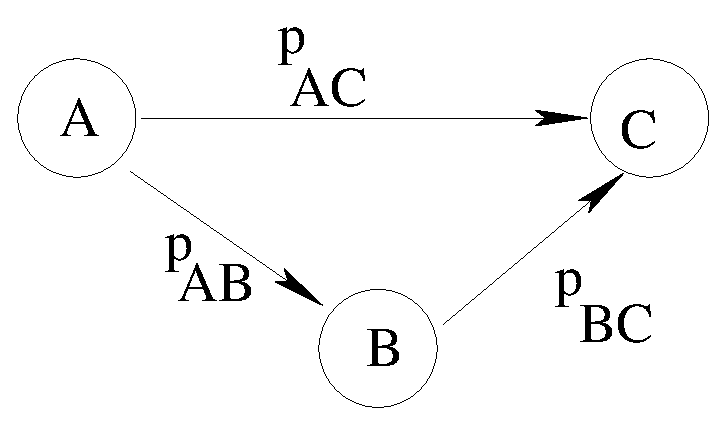
\includegraphics[width=0.4\linewidth]{routage.eps}
\end{center}

Vous devez transmettre un message d'un site  $A$ à  un site $C$.
Il y a deux chemins possibles~: le chemin direct $A \rightarrow C$,
et le chemin $A \rightarrow B \rightarrow C$. La probabilité de 
perte du message est $p_{AC}$ le long de l'arc $A \rightarrow C$,
$p_{AB}$ le long de l'arc $A \rightarrow B$, 
et $p_{BC}$ le long de l'arc $B \rightarrow C$. 
Vous noterez $r_{AC}=1-p_{AC}$
la  probabilité de réussite le long de l'arc $A \rightarrow C$. Idem pour
$r_{AB}=1-p_{AB}$ et $r_{BC}=1-p_{BC}$.
Quelles  sont les probabilités de perte et  de réussite du message sur le chemin $A \rightarrow B \rightarrow C$~?


%3. Avec quels coûts étiqueter les arcs d'un graphe pour réduire le calcul du chemin le plus fiable à un problème de chemin le plus court~? La justification n'est pas demandée.

\section{Arbre et jeu, algorithme du min-max}

Plusieurs jeux à deux joueurs  (dames, échecs, othello)
peuvent en théorie  être représentés ainsi par un arbre\footnote{En fait, il s'agit d'un graphe orienté sans cycle~: des sommets peuvent être partagés.}~: 
la situation courante  est décrite par un pion qui se trouve sur un sommet de l'arbre, initialement s1 sur la figure. A commence et peut déplacer le pion en s2 ou s3, disons s2. Ensuite $B$ joue, et doit déplacer le pion sur un sommet voisin de s2, soit s4, soit s5.
Un sommet du jeu est représenté par un rectangle quand c'est à A de jouer,
et par une ellipse quand c'est à B de jouer.

\begin{center}
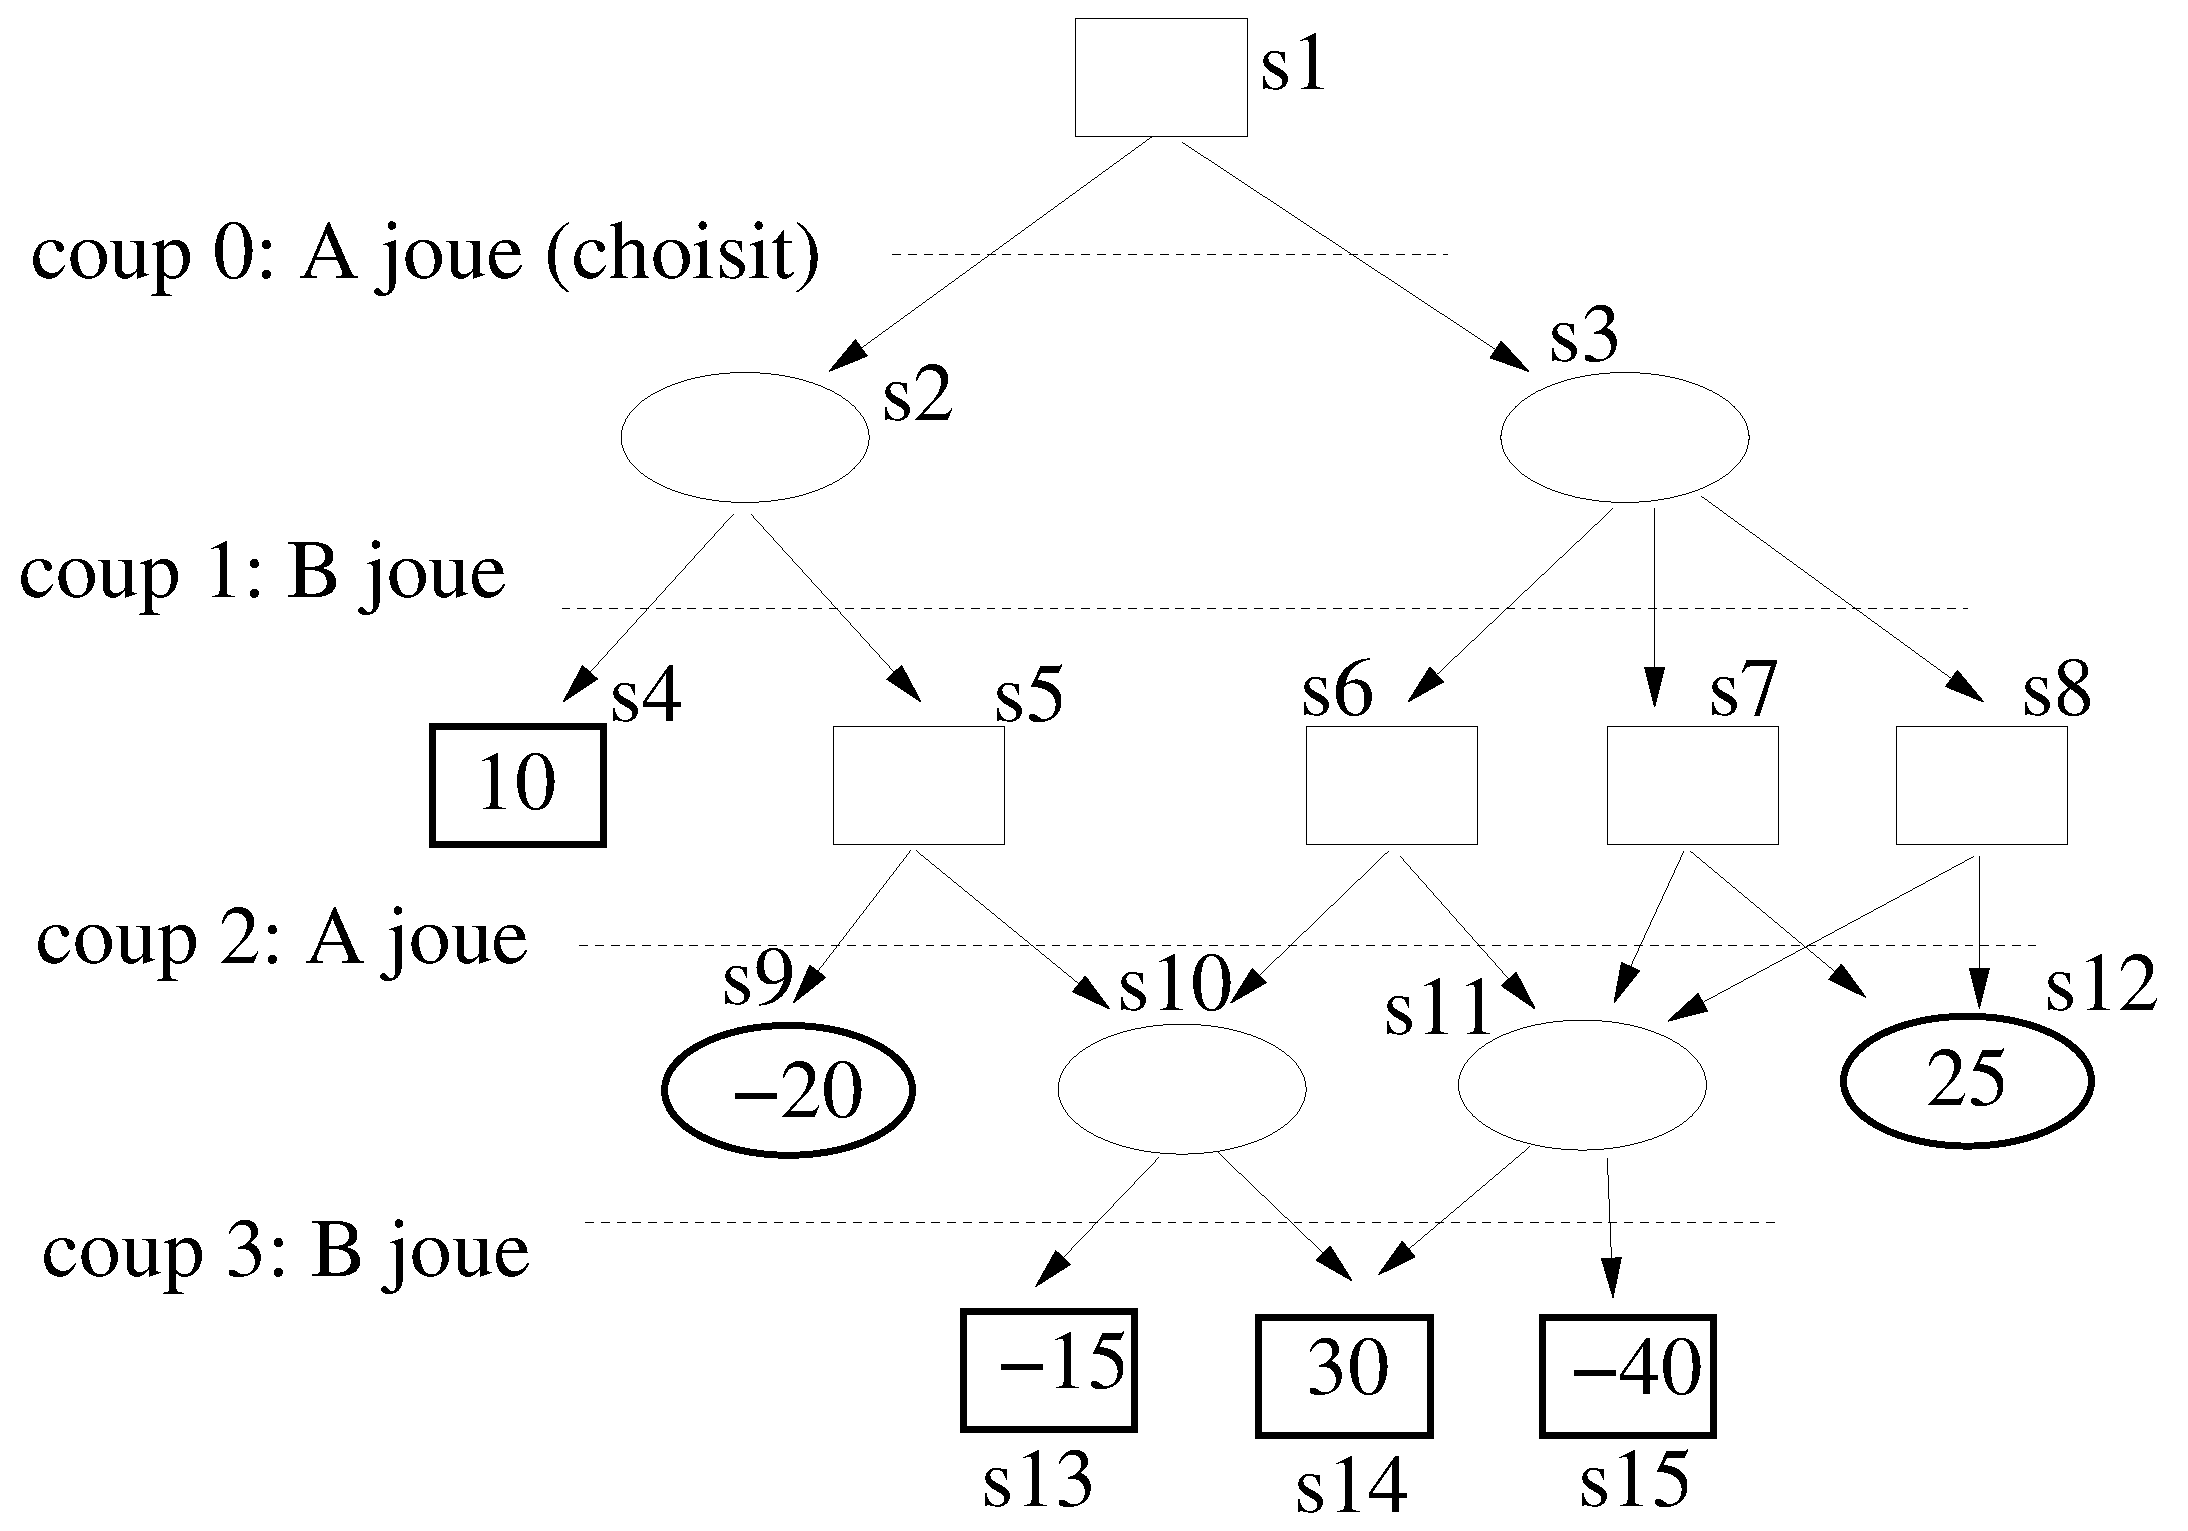
\includegraphics[width=0.95\linewidth]{jeu.eps}
\end{center}

Si le sommet n'a pas de voisin, il est dit terminal~; 
tout sommet terminal, qu'il soit rectangle ou ellipse,
est étiqueté par sa "valeur", par convention le gain de $B$, autrement dit  
la somme que $A$ doit payer à $B$ quand le jeu s'y termine. 

Cette valeur est donc positive quand $B$ gagne, et négative quand $B$ perd.  
Bien sûr, $B$ veut maximiser cette valeur (donc la valeur en s10 est 30), et $A$ veut 
la minimiser (donc la valeur en s5 est -20). 


Comme vous, A et B connaissent le graphe~; s'ils jouent tous les deux parfaitement, qui va gagner et combien~? Décrivez votre algorithme en 2 lignes maximum, et 
indiquez sur une figure 
les valeurs des sommets non étiquetés.

Pourquoi cette méthode n'est-elle pas utilisée pour des jeux de plateau (où toute l'information pertinente est connue des deux joueurs) tels que les dames, le jeu d'échec, Othello, Reversi, etc~? 

\section*{Fin de l'énoncé}
\newpage

 
\newpage

{\bf\LARGE Correction}
\maketitle
\section{Euclide et Bézout}

Pour $a=108, b=46$.

Rappel des formules~: si à une ligne, il y a~: $a$, $b$, $q$, $r$, $g$, $u$, $v$, alors à la ligne suivante il y a~: $a'=b$, $b'=r$, ... $g'=g$, $u'$ et $v'$.
Donc~:  $a=bq+r$, $bu'+rv'=g$ et $au+bv=g$. Donc
$u=v'$ et $v=u'-qv'$.
Ceci permet de remonter les valeurs de $u$ et $v$, du bas du tableau vers le haut.

$$\begin{array}{|c|c|c|c|c|c|c|}
\hline
a & b & a\div b & a\mod b & g &u & v \\
\hline
108 & 46 & 2 & 16 & 2 & 3-23k & -7+54k \\
46 & 16  & 2 & 14 & 2 & -1+8k & 3-23k  \\
16 & 14  & 1 & 2  & 2 & 1-7k  & -1+8k  \\
14  & 2  & 7 & 0  & 2 & k     & 1-7k  \\
2  & 0   & * & *  & 2 & 1     & k  \\
\hline
\end{array}
$$

\section{Dates au plus tôt et au plus tard}
\begin{center}
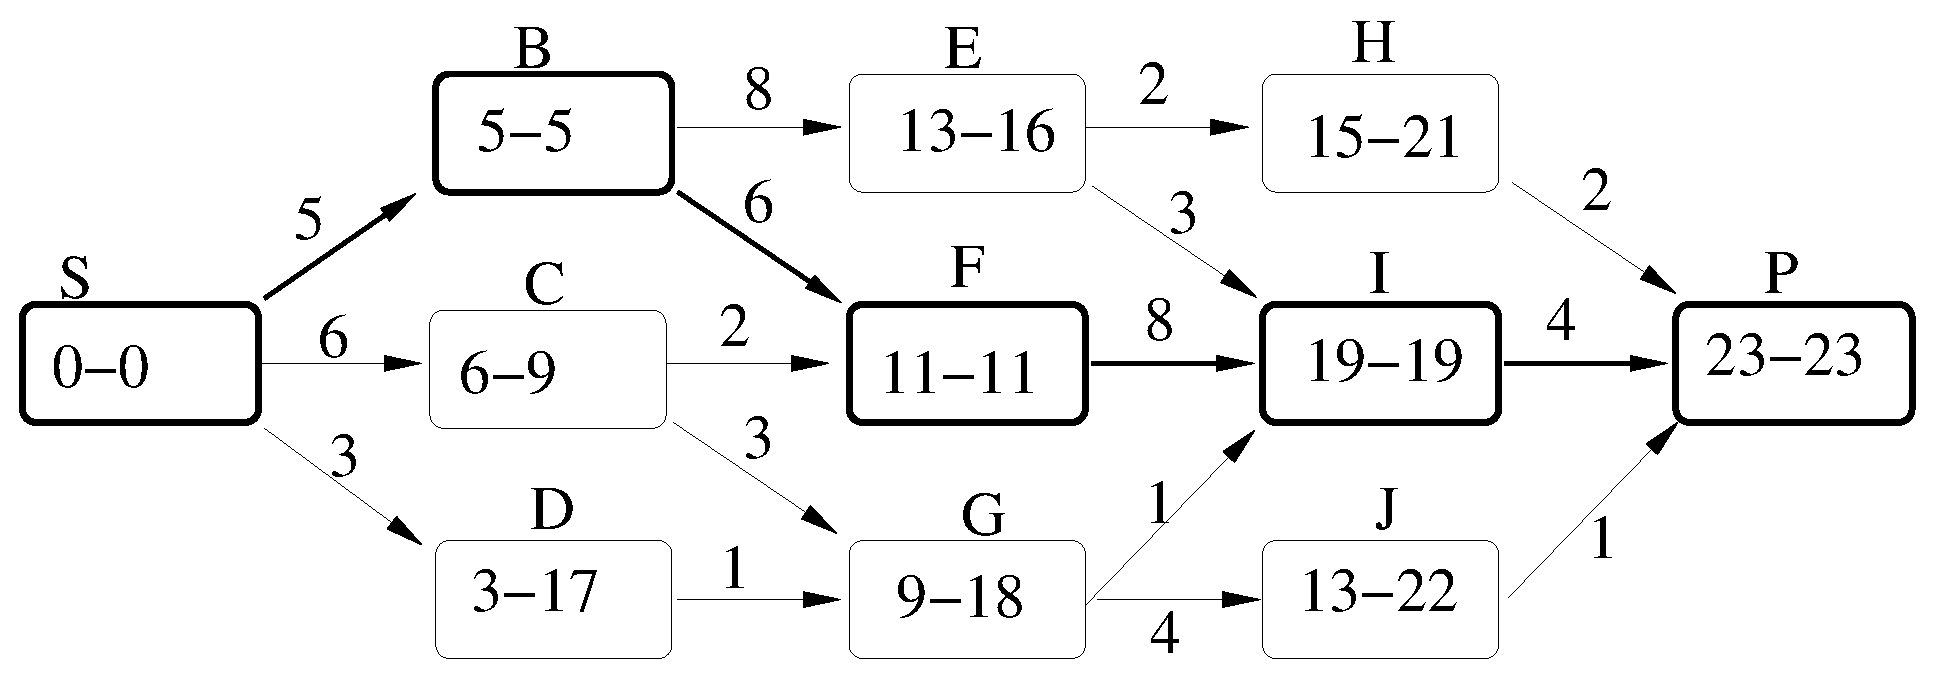
\includegraphics[width=0.95\linewidth]{critic_solution.eps}
\end{center}

\section{Quizz}

1. Problèmes difficiles mais décidables. 3-SAT, clique ou stable max, chemin hamiltinien, voyageur de commerce, MAX-SAT, tous les problèmes NP-complets.

2....

3. Backtrack. Traversée (ou parcours) en largeur (ou en largeur d'abord, "breadth first search") obtenue quand la structure d'attente utilisée est une file. Traversée en profondeur ou en profondeur d'abord("depth first search") obtenue quand la structure d'attente utilisée est une pile.

4. liste, pile, file, arbre, DAG (directed acyclic graph), graphe, table de hachage ("hash table").

\section{Fibonacci}

Q1. Intérêt de la définition matricielle de $F_n$~: la puissance rapide permet de calculer $F_n$ rapidement~:  elle n'a pas à calculer tous les termes précédents de la suite.
Elle effectue $O(\log n)$ produits de matrices $2\times 2$, alors que l'algorithme qui calcule tous les termes est en $O(n)$.

Q3. $T_n = a_{2}T_{n-2} + a_1T_{n-1}+ a_0$
$$\left(\begin{array}{c} T_{n-1}  \\
T_{n}\\
1 \end{array}\right)=
\left(\begin{array}{ccc} 
0 & 1 & 0 \\
a_2 & a_1 & a_0 \\
0 & 0 & 1 \end{array}\right)\left(\begin{array}{c} T_{n-2}  \\
 T_{n-1} \\
1 \end{array}\right) 
=\ldots = \left(\begin{array}{ccc}
0 & 1 & 0 \\
a_2 & a_1 & a_0 \\
0 & 0 & 1 \end{array}\right)^{n-1}\left(\begin{array}{c} T_{0} \\
T_1 \\
1  \end{array}\right)
$$

Q4. Supposons pour simplifier qu'il y a l'égalité~: $F_n = \phi^n / \sqrt{5}$. Alors~: $$\log( F_n) = \log(\phi^n / \sqrt{5}) = n \log\phi - \log(\sqrt{5}) \Rightarrow  n= (\log F_n+\log\sqrt{5})/\log\phi   $$ 

\section{Routage de message}


1. La probabilité  de réussite du message sur le chemin $A \rightarrow B \rightarrow C$ est~:

$$r_{ABC} = r_{AB} \times r_{BC}$$ 

$$p_{ABC}= 1 - r_{ABC}=1 - (1-p_{AB})(1-p_{BC})$$

Le dessin suivant permet de trouver facilement les probabilités de tous les chemins~; la probabilité d'un chemin est le produit des probabilités de ses arcs.
En chaque sommet, la somme des probabilités des arcs sortants vaut 1.

\begin{center}
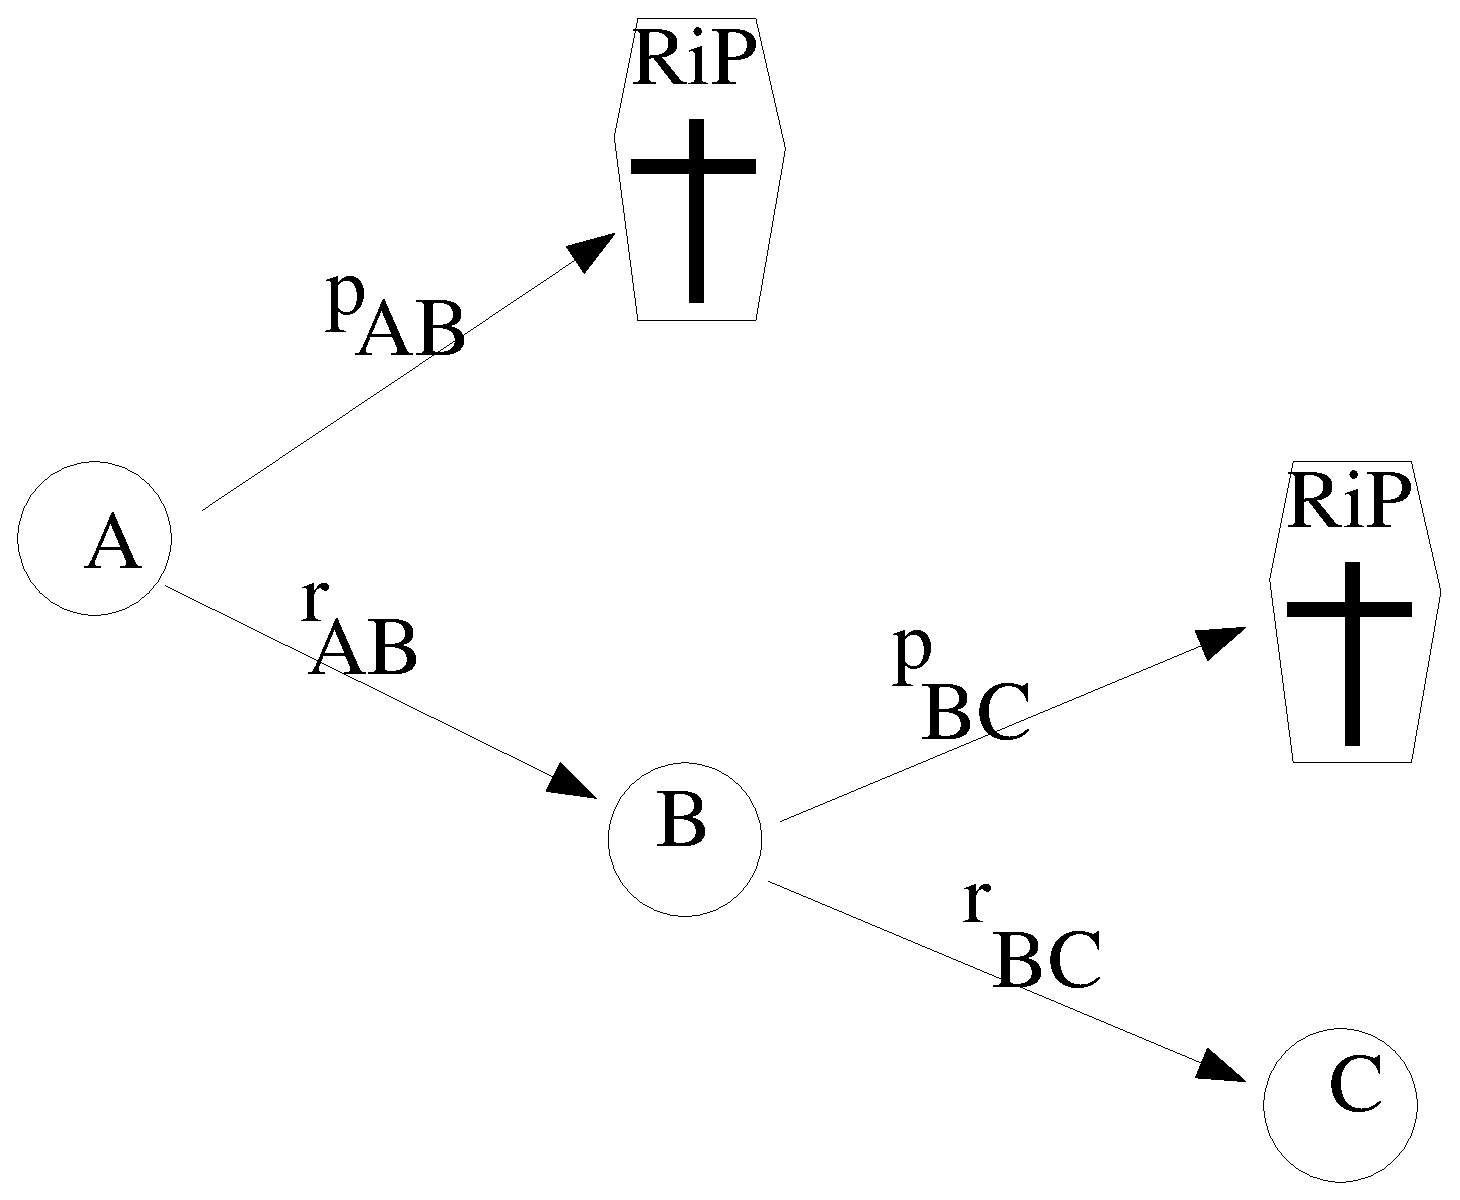
\includegraphics[width=0.5\linewidth]{ABC.eps}
\end{center}

3. Expliquez de façon claire et concise
comment vous pouvez réduire le calcul du chemin le plus fiable à un problème de chemin le plus court en moins de 5 lignes.

Etiqueter les arcs par le logarithme de l'inverse de leur (probabilité de) réussite, et chercher le chemin le plus court entre le départ et l'arrivée dans ce graphe.

Preuve (non demandée). La réussite d'un chemin est le produit des réussites de ses arcs. Maximiser le produit des réussites équivaut à maximiser son logarithme ($\log$ est  croissant), donc à maximiser la somme des logarithmes des réussites des  arcs du chemin. Ces logarithmes sont négatifs (car les réussites sont dans $(0, 1]$). Cela équivaut à minimiser l'opposé, donc à minimiser la somme des inverses des réussites.

 $$ \max \prod_{ij} r_{ij} \equiv \max \log (\prod_{ij} r_{ij}) =\max \sum_{ij} \log r_{ij} = - \min( -\sum_{ij}\log r_{ij}) $$
$$\min( -\sum_{ij} \log r_{ij}) = \min \sum_{ij}(-\log r_{ij})=\min \sum_{ij} \log(1/r_{ij})$$


\section{Arbre et jeu}
Les valeurs sont remontées des sommets terminaux vers la racine de l'arbre.
C'est possible car le graphe est acyclique (et fini, et discret).
B choisit le sommet voisin de valeur max~: la valeur d'un sommet rectangulaire
est le min des valeurs des sommets voisins (c'est A qui choisit, et il 
veut minimiser ses pertes), et la valeur d'un sommet elliptique est le max des valeurs des sommets voisins (c'est B qui choisit et il veut maximiser ses gains, \ie la valeur du jeu). 
Le jeu a comme valeur 10, donc si A et B jouent parfaitement, B gagne 10 et A perd 10. 

\begin{center}
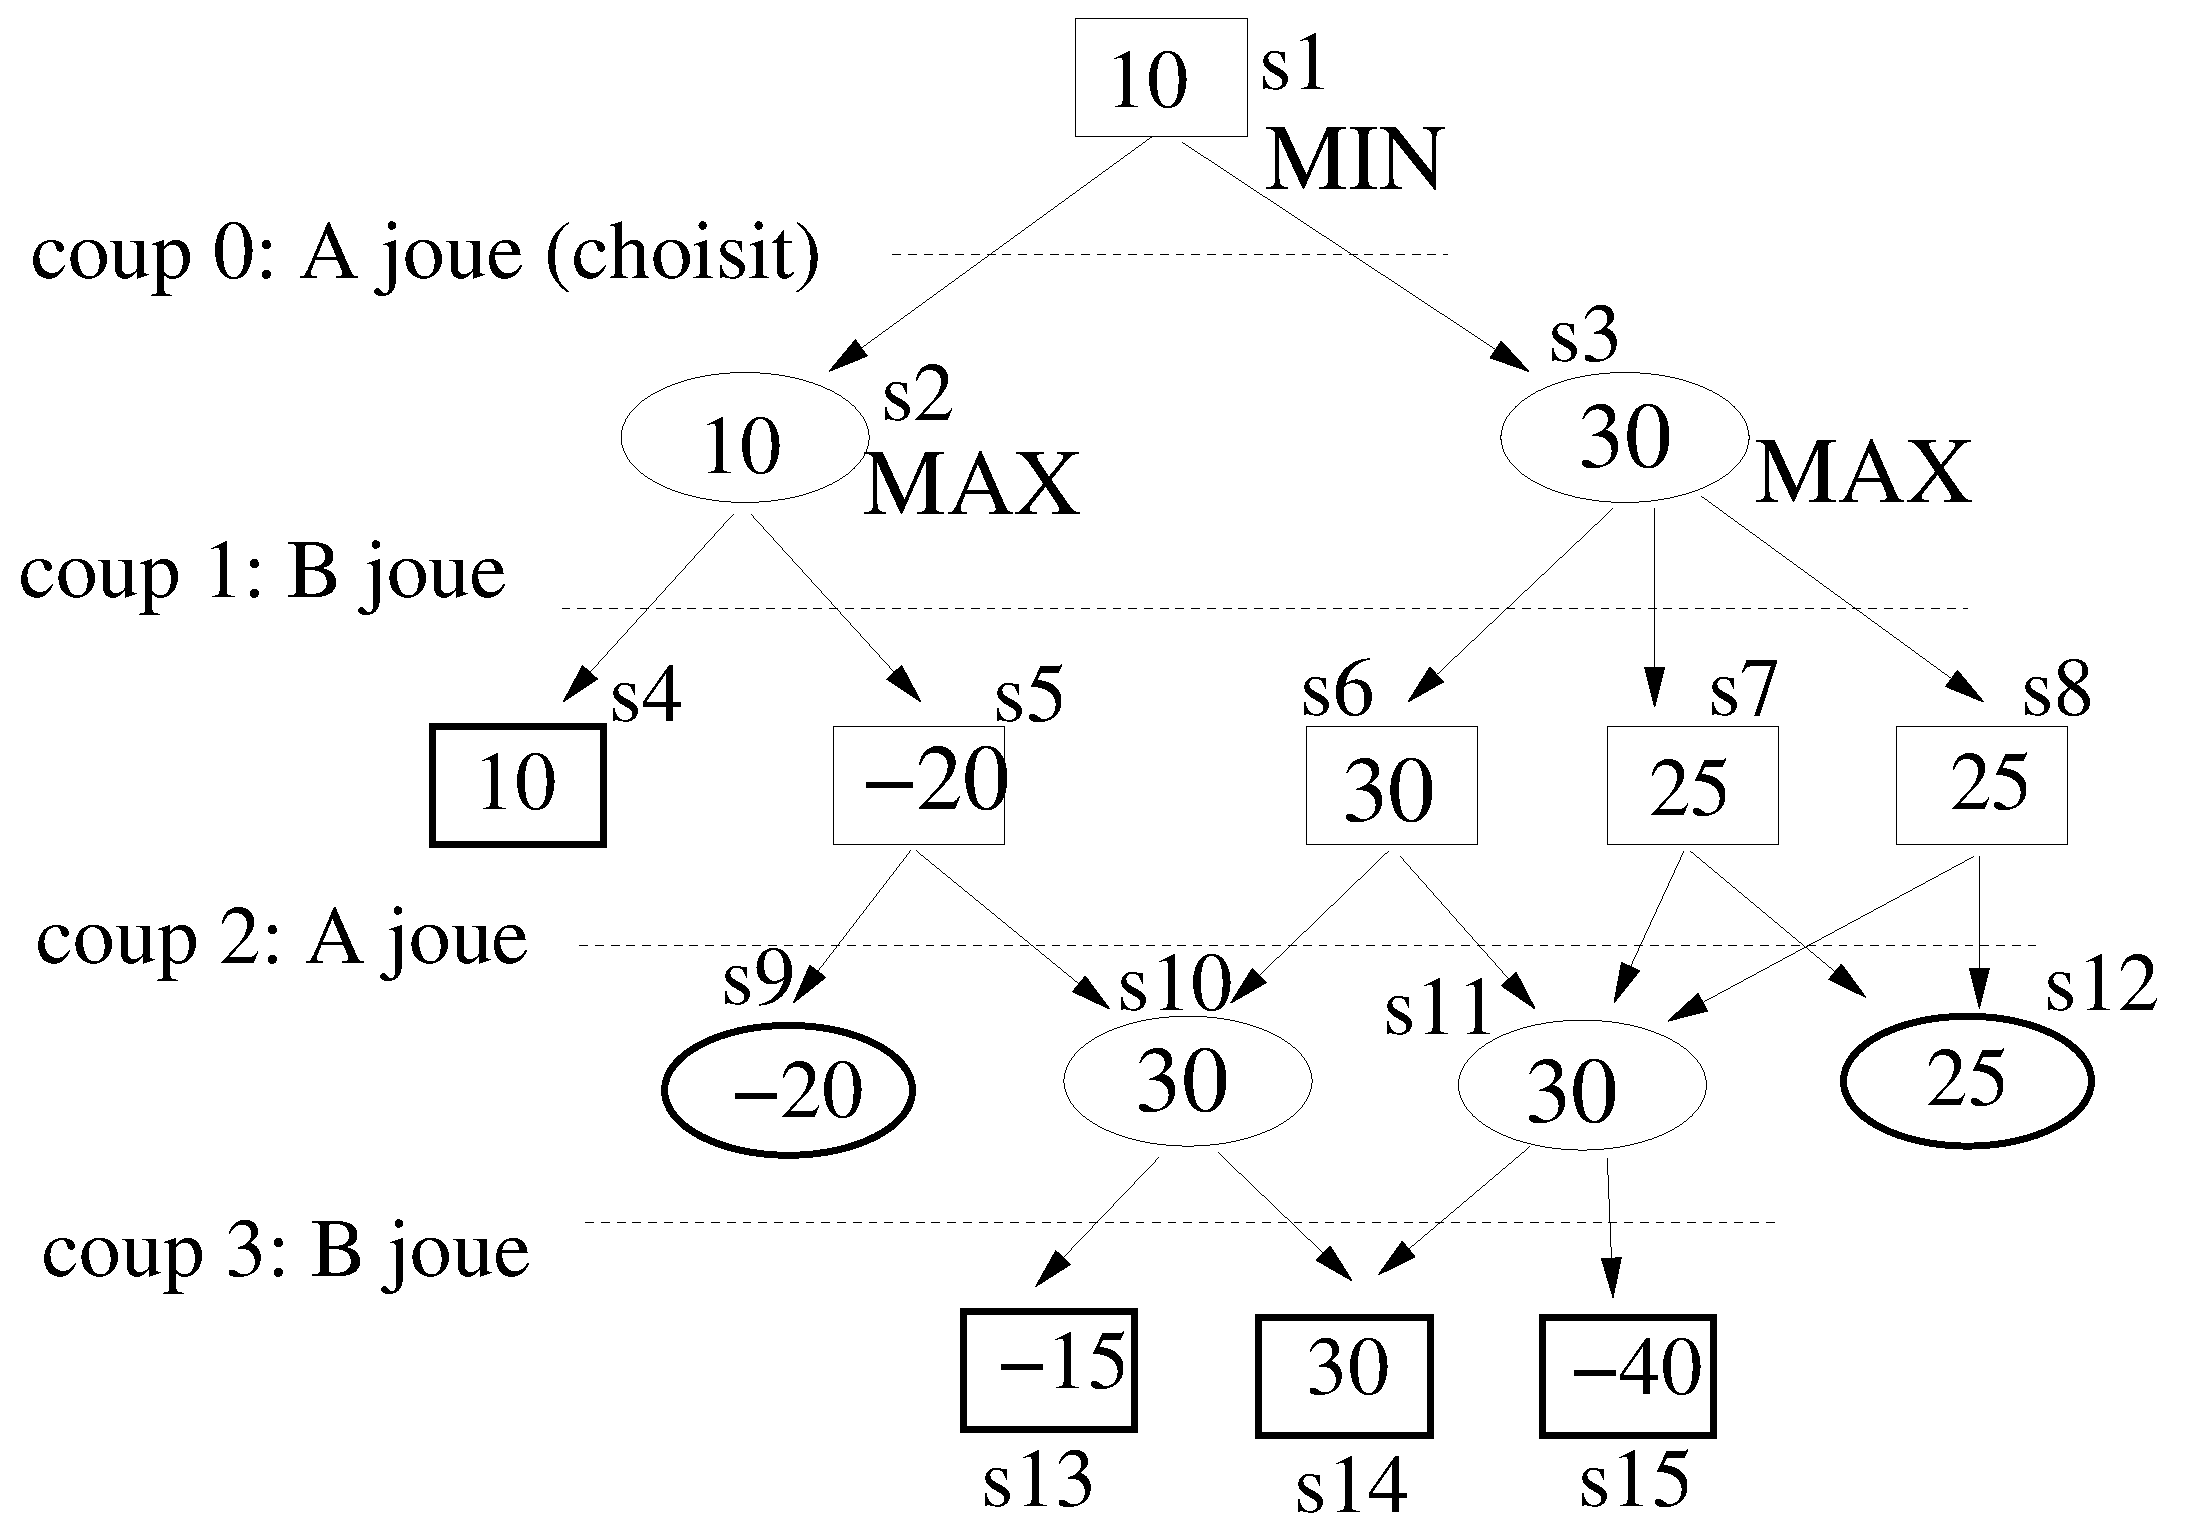
\includegraphics[width=0.99\linewidth]{jeu_solution.eps}
\end{center}
Cette méthode ne peut pas être utilisée sur de "vrais" jeux, car la taille du graphe est colossale. Il faut se contenter d'approximations, telles le
minimax avec élagage alpha-béta. 

Sur cette figure, les disques sont des positions gagnantes~; chaque disque émet une demi-droite horizontale, une demi-droite verticale et une demi-droite diagonale de points perdants.


\end{document}
{
\section{Un autre jeu}

Deux joueurs jouent à tour de rôle. Sur la table, il y a deux tas de pions.
Chaque joueur peut soit retirer un ou des pions dans un seul des tas, n'importe lequel, soit retirer le même nombre de pions dans les deux tas.
Aucun joueur  ne peut  retirer plus de pions qu'il n'y en a.
Le joueur qui retire le dernier pion a gagné.

L'état du jeu peut être représenté par $(a, b)$ où $a$ et $b$ sont le nombre de pions dans les deux tas. $(a, b)$ est équivalent à $(b, a)$.
Par définition, l'état $(0, 0)$ est gagnant, sous-entendu~: pour le joueur qui arrive à cet état~; donc les états $(0, p)$ ou $(p, 0)$ ou  $(p, p)$ ("sur la diagonale") avec $p \ge 1$  sont tous perdants. 

Dessinez la grille des points entiers $(a, b)$ et marquez-y les états gagnants,
avec $ 0 \le a \le 7$, $0\le  b\le 7$.


\begin{center}
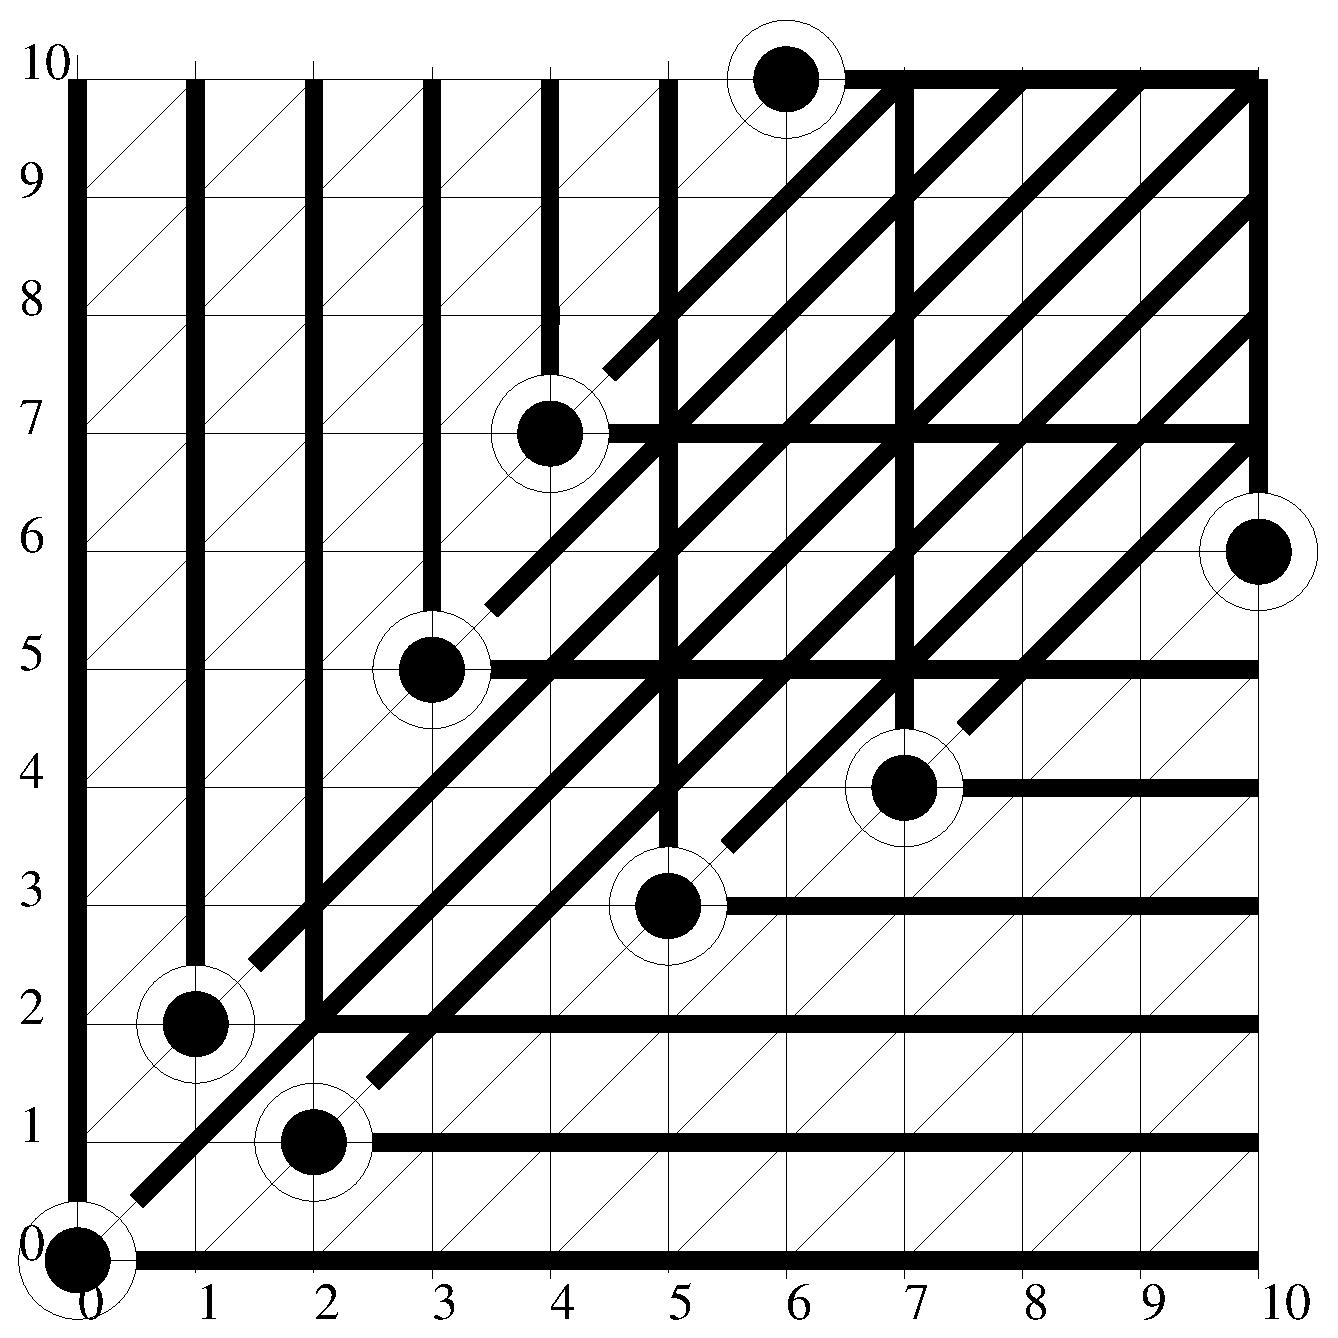
\includegraphics[width=0.95\linewidth]{nim_autre.eps}
\end{center}
}
